\section{lg\-Sequence Class Reference}
\label{classlgSequence}\index{lgSequence@{lgSequence}}
a {\bf lg\-Voice} used as GUIDO Sequence  


{\tt \#include $<$lgsequence.h$>$}

Inheritance diagram for lg\-Sequence::\begin{figure}[H]
\begin{center}
\leavevmode
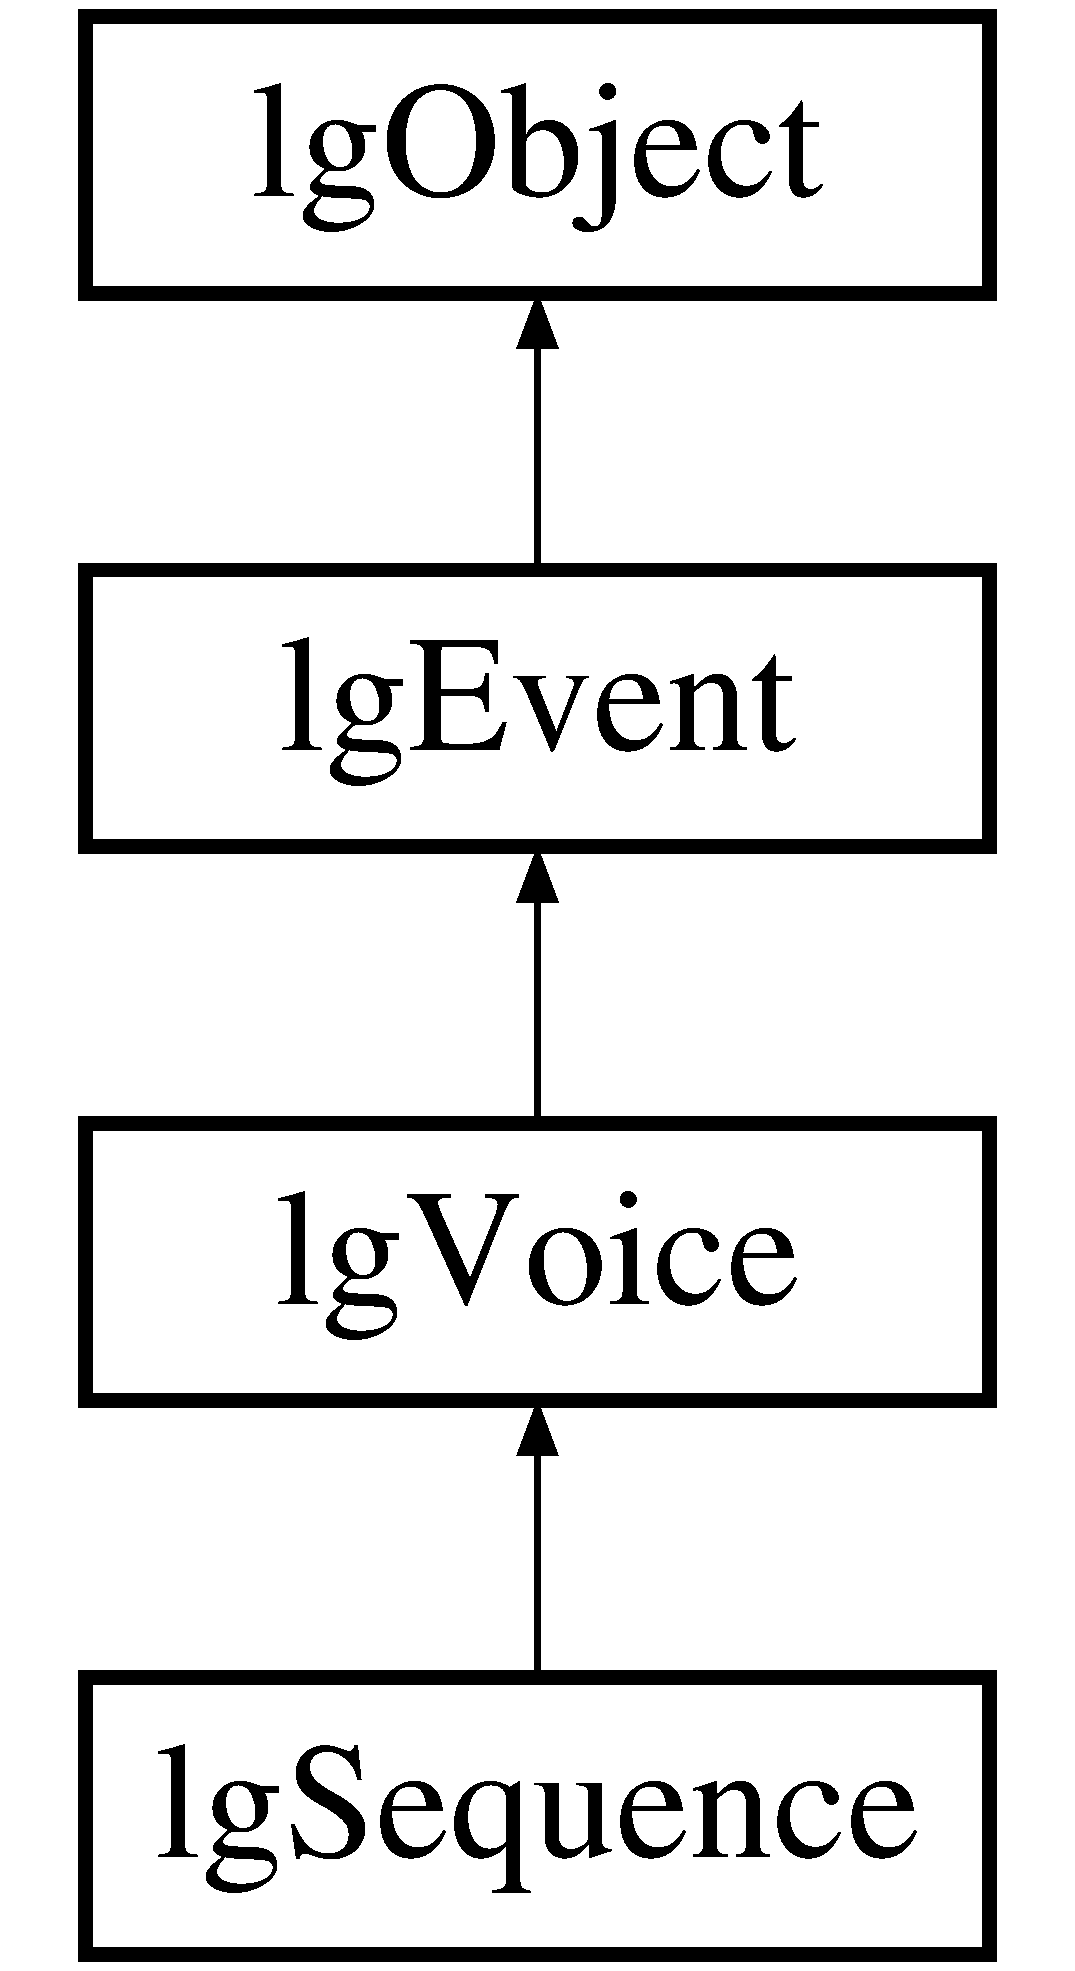
\includegraphics[height=4cm]{classlgSequence}
\end{center}
\end{figure}
\subsection*{Public Member Functions}
\begin{CompactItemize}
\item 
virtual string {\bf to\-String} ({\bf lg\-Voice} $\ast$calling\-Seq=NULL)
\item 
{\bf lg\-Sequence} (long int pos\-Num, long int pos\-Denom)
\item 
void {\bf set\-ID} (int id)
\item 
int {\bf get\-ID} (void)
\end{CompactItemize}
\subsection*{Private Attributes}
\begin{CompactItemize}
\item 
int {\bf ID}
\end{CompactItemize}


\subsection{Detailed Description}
a {\bf lg\-Voice} used as GUIDO Sequence 



\subsection{Constructor \& Destructor Documentation}
\index{lgSequence@{lg\-Sequence}!lgSequence@{lgSequence}}
\index{lgSequence@{lgSequence}!lgSequence@{lg\-Sequence}}
\subsubsection{\setlength{\rightskip}{0pt plus 5cm}lg\-Sequence::lg\-Sequence (long int {\em pos\-Num}, long int {\em pos\-Denom})}\label{classlgSequence_a1}




\subsection{Member Function Documentation}
\index{lgSequence@{lg\-Sequence}!getID@{getID}}
\index{getID@{getID}!lgSequence@{lg\-Sequence}}
\subsubsection{\setlength{\rightskip}{0pt plus 5cm}int lg\-Sequence::get\-ID (void)}\label{classlgSequence_a3}


\index{lgSequence@{lg\-Sequence}!setID@{setID}}
\index{setID@{setID}!lgSequence@{lg\-Sequence}}
\subsubsection{\setlength{\rightskip}{0pt plus 5cm}void lg\-Sequence::set\-ID (int {\em id})}\label{classlgSequence_a2}


\index{lgSequence@{lg\-Sequence}!toString@{toString}}
\index{toString@{toString}!lgSequence@{lg\-Sequence}}
\subsubsection{\setlength{\rightskip}{0pt plus 5cm}string lg\-Sequence::to\-String ({\bf lg\-Voice} $\ast$ {\em calling\-Seq} = NULL)\hspace{0.3cm}{\tt  [virtual]}}\label{classlgSequence_a0}


tags at beginn of the voice 

write event

write all tags after event 

Reimplemented from {\bf lg\-Voice} {\rm (p.\,\pageref{classlgVoice_a20})}.

\subsection{Member Data Documentation}
\index{lgSequence@{lg\-Sequence}!ID@{ID}}
\index{ID@{ID}!lgSequence@{lg\-Sequence}}
\subsubsection{\setlength{\rightskip}{0pt plus 5cm}int {\bf lg\-Sequence::ID}\hspace{0.3cm}{\tt  [private]}}\label{classlgSequence_r0}




The documentation for this class was generated from the following files:\begin{CompactItemize}
\item 
{\bf lgsequence.h}\item 
{\bf lgsequence.cpp}\end{CompactItemize}
